\documentclass[twoside,10pt]{article}
\usepackage{/Users/bradenhoagland/latex/styles/toggles}
%\toggletrue{sectionbreaks}
%\toggletrue{sectionheaders}
\newcommand{\docTitle}{Math 412 - HW 7}
\usepackage{/Users/bradenhoagland/latex/styles/common}
\importStyles{modern}{rainbow}{boxy}

\newcommand{\dgm}{\text{dgm}}

\begin{document}
%\tableofcontents

%--------------------------------------------------------------------------------
% problem 1
%--------------------------------------------------------------------------------
\begin{exer}[Lesson 12, 5 points]
	Prove $d_I$, the interleaving distance, satisfies the triangle inequality. That is, for any persistence modules $P$, $Q$, and $R$ prove
	\[
	d_I(P, Q) \leq d_I(P, R) + d_I(R, Q).
	\]
	Prove that if $P$ and $Q$ have an $\epsilon$-interleaving and $\delta > \epsilon$ then $P$ and $Q$ also have a $\delta$-interleaving.
\end{exer}

\textbf{$\delta$ interleaving:} First we will show that for all $\delta>\varepsilon$, there is a $\delta$-interleaving. We need to show that the four diagrams commute; we'll start with the following.

\begin{figure}[H]
	\centering
	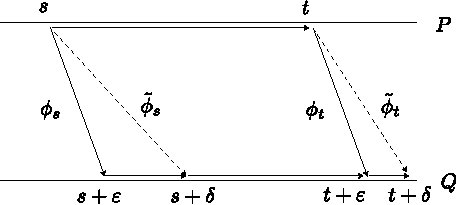
\includegraphics[scale=1]{fig/1a.pdf}
	%\caption{}
\end{figure}

Consider the compositions $\tilde{\phi}_s := Q_{s+\varepsilon}^{s+\delta}\phi_s$ and $\tilde{\phi}_t := Q_{t+\varepsilon}^{t+\delta}\phi_t$. These make the diagram commute since
\begin{align*}
	\tilde{\phi}_t P_{s}^{t} &= Q_{t+\varepsilon}^{t+\delta}\phi_t P_{s}^{t} \\
				 &= Q_{t+\varepsilon}^{t+\delta} Q_{s+\varepsilon}^{t+\varepsilon} \phi_s \\
				 &= Q_{s+\varepsilon}^{t+\varepsilon}\phi_s \\
				 &= Q_{s+\delta}^{t+\delta} Q_{s+\varepsilon}^{s+\delta}\phi_s \\
				 &= Q_{s+\delta}^{t+\delta} \tilde{\phi}_s.
\end{align*}

\begin{figure}[H]
	\centering
	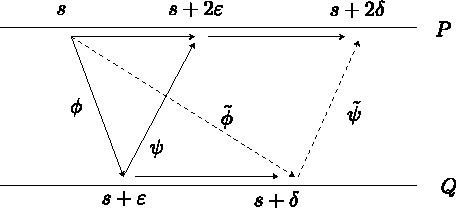
\includegraphics[scale=1]{fig/1b.pdf}
	%\caption{}
\end{figure}

Consider the maps $\tilde{\phi} := Q_{s+\varepsilon}^{s+\delta}\phi_s$ and
\[
	\tilde{\psi} :=
	\begin{cases}
		P_{s+2\varepsilon}^{s+2\delta} \psi_{s+\varepsilon} & \text{ on } Q_{s+e}^{s+\delta}(Q_{s+e}), \\
		0 & \text{ elsewhere}.
	\end{cases}
\] 
The map $\tilde{\psi}$ is well-defined since $P_{x}^{y}$ and $Q_{s}^{y}$ are either inclusions or zero maps for all $x,y$. Note that $\tilde{\psi}$ satisfies $\tilde{\psi} Q_{s+\varepsilon}^{s+\delta} = P_{s+2\varepsilon}^{s+2\delta}\psi_{s+\varepsilon}$. These two maps then make the diagram commute:
\begin{align*}
	\tilde{\psi} \tilde{\phi} &= \tilde{\psi} Q_{s+\varepsilon}^{s+\delta} \phi_s \\
				  &= P_{s+2\varepsilon}^{s+2\delta} \psi_{s+\varepsilon} \phi_s \\
				  &= P_{s+2\varepsilon}^{s+2\delta} P_{s}^{s+2\varepsilon} \\
				  &= P_{s}^{s+2\delta}.
\end{align*}
The proofs for the other two diagrams are almost identical: just swap each $\phi$ and $\psi$ and swap each $P$ and $Q$ from the above two proofs. Thus if there is an $\varepsilon$-interleaving, then for all $\delta>\varepsilon$, there is also a $\delta$-interleaving.

\textbf{Triangle Inequality:} Now we will show that $d_I$ satisfies the triangle inequality. Suppose $d_I(P,R)=\tilde{\varepsilon}$ and $d_I(R,Q) = \tilde{\delta}$, then we want to show that $d_I \leq \tilde{\varepsilon}+\tilde{\delta}$. By the previous part of the problem, we know that for all $\varepsilon>\tilde{\varepsilon}$ and $\delta>\tilde{\delta}$, there is an $\varepsilon$-interleaving between $P$ and $R$ and a $\delta$-interleaving between $R$ and $Q$. For all $\varepsilon$ and $\delta$, we will find an $(\varepsilon+\delta)$-interleaving between $P$ and $Q$.

Fix $\varepsilon$ and $\delta$, then we can do the same analysis on 2 of the 4 diagrams.

\begin{figure}[H]
	\centering
	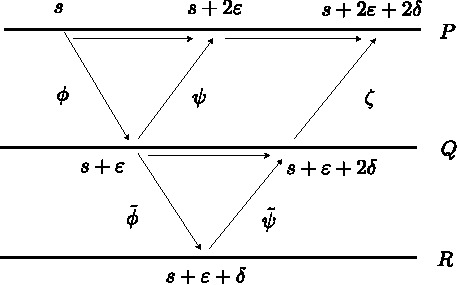
\includegraphics[scale=1]{fig/1c.pdf}
	%\caption{}
\end{figure}

In the above diagram, the quadrilateral and both inner triangles commute because of the $\varepsilon$ and $\delta$ interleavings. Thus the outer triangle also commutes:
\begin{align*}
	\zeta \tilde{\psi} \tilde{\phi} \phi &= \zeta Q_{s+\varepsilon}^{s+\varepsilon+2\delta}\phi \\
					     &= P_{s+2\varepsilon}^{s+2\varepsilon+2\delta}\psi \phi \\
					     &= P_{s+2\varepsilon}^{s+2\varepsilon+2\delta}P_{s}^{s+2\varepsilon} \\
					     &= P_{s}^{s+2\varepsilon+2\delta}.
\end{align*}

\begin{figure}[H]
	\centering
	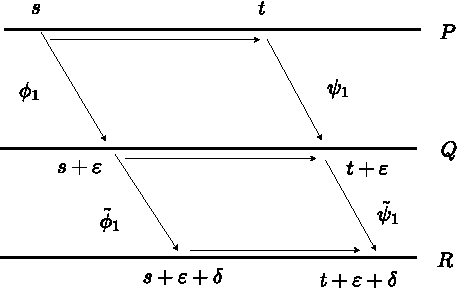
\includegraphics[scale=1]{fig/1d.pdf}
	%\caption{}
\end{figure}

In the above diagram, both inner quadrilaterals commute because of the $\varepsilon$ and $\delta$ interleavings. Then the outer quadrilateral also commutes:
\begin{align*}
	Q_{s+\varepsilon+\delta}^{t+\varepsilon+\delta} \tilde{\phi}_1 \phi_1 &= \tilde{\phi}_2 R_{s+\varepsilon}^{t+\varepsilon} \phi_1 \\
									      &= \tilde{\phi}_2 \phi_2 P_{s}^{t} \\
									      &= \tilde{\phi}_2 \phi_2 P_{s}^{t}.
\end{align*}
Since $\varepsilon$ and $\delta$ can be made arbitrarily close to $\tilde{\varepsilon}$ and $\tilde{\delta}$, we know $d_{I}(P,Q) \leq \tilde{\varepsilon}+\tilde{\delta}$, as desired.


\newpage

%--------------------------------------------------------------------------------
% problem 2
%--------------------------------------------------------------------------------
\begin{exer}[Lesson 12, 10 points]
	Suppose $P$ and $Q$ are persistence modules. Prove
	\[
	d_B(\dgm(P), \dgm(Q)) \geq d_I(P, Q).
	\]
	Hint: First, check that you can  pad a persistence module by the zero module and preserve its isomorphism type, that is, $P \oplus 0 \cong P$. Second, prove the statement for interval modules. Third, apply a careful induction on the number of intervals in $P$ and $Q$.
\end{exer}

\textbf{Part I:} We will first show that for any persistence module $P$, we have $P \oplus 0 \cong P$. Consider the linear maps $\phi_t:P_t \to P_t \oplus 0$ given by $p \mapsto (p,0)$. These are clearly bijective, so since they are linear, this is enough to be an isomorphism. Now we just have to show that they respect the inclusions of the persistence modules. This means that the following diagram commutes for all $s$ and $t$, where $Q := P \oplus 0$ is the persistence module with vector spaces $Q_t := P_t$ and inclusions $Q_{s}^{t} := (P_s^t, 0)$.

\[
\begin{tikzcd}
	P_s \rar{P_{s}^{t}}\dar[shift left]{\phi_s} & P_{t} \dar[shift left]{\phi_t} \\
	Q_s \uar[shift left]{\phi_{s}^{-1}} \rar["Q_{s}^{t}"'] & Q_t \uar[shift left]{\phi_t^{-1}}
\end{tikzcd}
\] By the definitions of $Q$ and $\phi_t$,
\begin{align*}
	(\phi_t P_{s}^{t})(p) &= (P_{s}^{t}(p), 0) = (Q_{s}^{t} \phi_s)(p) \text{ and}\\
	(P_{s}^{t}\phi_{s}^{-1})(q,0) &= P_{s}^{t}(q) = (\phi_{t}^{-1}Q_{s}^{t})(q, 0)
\end{align*}
for all $p, q \in P$, so the diagram commutes. Thus $P \cong P \oplus 0$ as persistence modules.

\textbf{Part II:} We'll now show that the theorem holds if $P$ and $Q$ are interval modules. Suppose $P = I_{[a,b)}$ and $Q = I_{[c,d)}$, then there are two possible partial matchings: they are either both matched or neither are matched. Let's suppose that $ (a,b)$ and $(c,d)$ \textit{are} matched by the optimal partial matching, then
\[
	{\Vert{(a,b)-(c,d)}\Vert}_{\infty} = \max\left\{ |a-c|, |b-d| \right\} =: \varepsilon.
\] 
Note that this implies $[a,b) \subseteq [c-\varepsilon,d+\varepsilon)$ and $[c,d) \subseteq [a-\varepsilon,b+\varepsilon)$. We can then construct an $\varepsilon$-interleaving between $P$ and $Q$ by defining
\begin{align*}
	\phi_t &=
	\begin{cases}
		\id_{} & \text{ if } Q_{s+\varepsilon}= \mathbb{Z}_2,\\
		0 & \text{otherwise}.
	\end{cases},\\
	\psi_t &=
	\begin{cases}
		\id_{} & \text{ if } P_{s+\varepsilon}=\mathbb{Z}_2,\\
		0 & \text{otherwise}.
	\end{cases}
\end{align*}
We have to show that the usual diagrams commute. As in the previous problem, we actually only need to show this for 2 of them.

\begin{figure}[H]
	\centering
	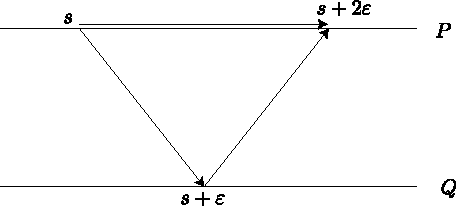
\includegraphics[scale=1]{fig/2a.pdf}
	%\caption{}
\end{figure}

If $P_s=0$, all involved maps are the zero map, so it must commute. Similarly, every map is 0 if $P_{s+2\varepsilon}=0$. We can then suppose that $P_{s}=P_{s+2\varepsilon}=\mathbb{Z}_2$, i.e. $s,s+2\varepsilon \in [a,b)$. Since $[a,b) \subseteq [c-\varepsilon,d+\varepsilon)$, we know
\begin{align*}
	s \in [a,b) &\implies [c,d+2\varepsilon),\\
	s+2\varepsilon \in [a,b) &\implies [c-\varepsilon,d).
\end{align*}
But this means $s+\varepsilon \in [c,d)$, so $Q_{s+\varepsilon}=\mathbb{Z}_2$, so all the involved maps are the identity. Thus the diagram commutes.

\begin{figure}[H]
	\centering
	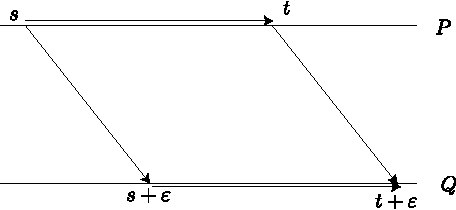
\includegraphics[scale=1]{fig/2b.pdf}
	%\caption{}
\end{figure}

If $P_s=0$ or $Q_{t+\varepsilon}=0$, then both compositions of maps are 0, so the diagram commutes. Thus we can suppose that both are $\mathbb{Z}_2$. Since $[a,b) \subseteq [c-\varepsilon,d+\varepsilon)$, a similar argument as for the previous diagram shows $s+\varepsilon \in [c,d)$. Thus $Q_{s+\varepsilon}=\mathbb{Z}_2$. We can similarly show $P_{t}=\mathbb{Z}_2$. Thus all involved maps are the identity, so the diagram commutes.

Now suppose $(a,b)$ and $(c,d)$ are \textit{not} matched by the optimal partial matching. This means $d_{B} = \max \left\{ \frac{b-a}{2} ,\frac{d-c}{2}  \right\} =: \varepsilon$. Without loss of generality, suppose $\varepsilon = \frac{b-a}{2} $, i.e. $(a,b)$ is farther from the diagonal than $(c,d)$.

We can represent this situation by matching $P$ and $Q$ with 0 modules. Using the same definitions of $\phi_t$ and $\psi_t$ as above, we can find $\varepsilon$-interleavings between $P$ and $0$ and between $Q$ and 0. We'll start with $P$.

\begin{figure}[H]
	\centering
	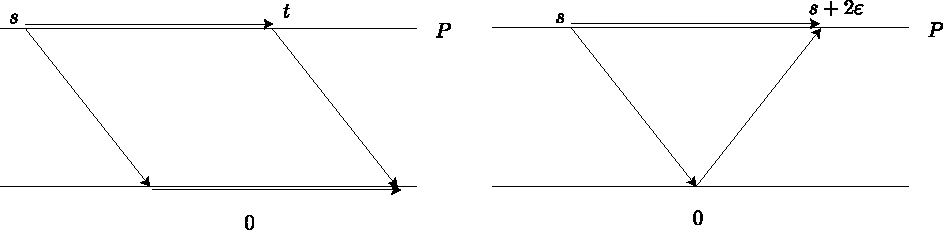
\includegraphics[scale=0.6]{fig/2c.pdf}
	%\caption{}
\end{figure}

For the triangle diagram, note that if $P_s=0$, then all the maps involved must be 0, and thus the diagram commutes. If $P_s = \mathbb{Z}_2$ instead, then since $2\varepsilon = b-a$, we necessarily have $P_{s+2\varepsilon}=0$, so the maps involved are once again all zero. For the quadrilateral diagram, since $Q_{t+\varepsilon}=0$, the two compositions we care about are both 0, so the diagram commutes. Thus $d_I(P,0) \leq \varepsilon$. Similarly, we can show $d_I(Q,0) \leq \frac{d-c}{2} \leq \varepsilon$.

\textbf{Part III:} We'll now extend the result from part II to arbitrary persistence modules $P$ and $Q$. Suppose $P$ and $Q$ have the following interval decomposition.
\[
	P \cong \bigoplus_{i=1}^{n} P_i, \qquad Q \cong \bigoplus_{i=1}^{m} Q_i.
\]
There are a finite number of partial matchings of $P$ and $Q$ since they both have a finite interval decomposition, so we can choose the partial matching $\eta$ with the lowest cost $c(\eta)$. Then $d_B = c(\eta)$.

The partial matching $\eta$ is a bijection $\phi:\left\{ 1, \dots, N \right\}\to \left\{ 1, \dots, N \right\}$ for some $N \geq \max\left\{ n,m \right\}$, i.e. we match $P_i$ with $Q_{\phi(i)}$ (the larger $N$ is because we might not match some of the $P_i$ and $Q_j$, so we'll need to add in some 0 modules to match the unmatched intervals with; by part I, this padding doesn't change $P$ or $Q$ up to isomorphism).
\begin{align*}
	P_1 &\oplus P_2 \oplus \cdots \oplus P_N \\
	Q_{\phi(1)} &\oplus Q_{\phi(s)} \oplus \cdots \oplus Q_{\phi(N)}
\end{align*}
Suppose the bottleneck distance between $P_i$ and $Q_{\phi(i)}$ is $\varepsilon_i$, then the cost of the matching $c(\eta)$ is $\varepsilon := \max_i \left\{ \varepsilon_i \right\}$. By part II, we know that there are $\varepsilon_i$-interleavings between $P_i$ and $Q_{\phi(i)}$ for all $i$. By part I, we can then find $\varepsilon$-interleavings between every $P_i$ and $Q_{\phi(i)}$. Finally, we can take the direct sum of all these interleavings to get an $\varepsilon$-interleaving between $P$ and $Q$ in their entirety. thus $d_I(P,Q) \leq \varepsilon = d_{B}$.

\end{document}
